\begin{name}
	{\tenchude}
	{TOÁN 12}
	{LỚP TOÁN THẦY PHÁT}
	{Thời gian: 90 phút - Không kể thời gian phát đề}
\end{name}
\TN
\Opensolutionfile{ans}[ans/ansDe1-TN1]
\begin{ex}%[2D4N1-1]%[Dự án EX-TF-TLN lần 3 -Mui Doan]
	Nguyên hàm của hàm số $f(x)=x^n$ (với $n\neq -1$) là
	\choice
	{\True $\dfrac{x^{n+1}}{n+1}+C$}
	{$x^{n+1}+C$}
	{$\dfrac{n+1}{x^{n+1}}+C$}
	{$\dfrac{1}{x^{n+1}}+C$}
	\loigiai{
		Nguyên hàm của hàm số $f(x)=x^n$ (với $n\neq -1$) là	$\dfrac{x^{n+1}}{n+1}+C$.
	}
\end{ex}

\begin{ex}%[2D4N1-1]%[Tổ 19 - Đợt 17 - Chương 4 - - CD - Đề 2]%[Bình]
	Hàm số $y=F(x)$ là một nguyên hàm của hàm số $y=f(x)$. Hãy chọn khẳng định \textbf{đúng}.
	\choice
	{$F(x)=f'(x)$}
	{\True $F'(x)=f(x)$}
	{$F(x)=f'(x)+C$}
	{$F'(x)+C=f(x)$}
	\loigiai
	{
		Khẳng định đúng là: $F'(x)=f(x)$.
	}
\end{ex}

\begin{ex}%[2D4N1-2]
	Họ nguyên hàm của hàm số $f(x)=3x^2+1$ là
	\choice
	{$x^3+C$}
	{$\dfrac{x^3}{3}+x+C$}
	{$6x+C$}
	{\True $x^3+x+C$}
	\loigiai{
		$\displaystyle\int{(3x^2+1)\mathrm{\,d}x=x^3+x+C}$.}
\end{ex}

\begin{ex}%[12-MH-2-MH2025]%[MH-2025,Chu Hà]%[2D4N1-3]
	Họ nguyên hàm của hàm số $f(x)= \dfrac{1}{\sqrt{x}} $ là
	\choice
	{\True $2\sqrt{x}+C$}
	{$\sqrt{x} + C$}
	{$- \sqrt{x} +C$}
	{$-2\sqrt{x}+C$}
	\loigiai
	{
	Ta có $\displaystyle \int\dfrac{1}{\sqrt{x}}\mathrm{\,d}x=\int x^{-\tfrac{1}{2}}\mathrm{\,d}x=2x^{\tfrac{1}{2}}+C=2\sqrt{x}+C$.
	}
\end{ex}

\begin{ex}%[2D4N1-4]
	Phát biểu nào sau đây là đúng?
	\choice
	{$\displaystyle\int e^{-3 x} \mathrm{~d} x=e^{-3 x}+C$}
	{\True $\displaystyle\int e^{-3 x} \mathrm{~d} x=-\frac{1}{3} e^{-3 x}+C$}
	{$\displaystyle\int e^{-3 x} \mathrm{~d} x=\frac{1}{3} e^{-3 x}+C$}
	{$\displaystyle\int e^{-3 x} \mathrm{~d} x=-\frac{1}{3} e^{-3 x}$}
	\loigiai{$\displaystyle\int e^{-3 x} \mathrm{~d} x=-\frac{1}{3} e^{-3 x}+C$.}
\end{ex}

\begin{ex}%[Dự án 2025 - đề cấu trúc mới, Nguyễn Kiều Nhã Tú]%[2D4N1-4]
	Họ nguyên hàm của hàm số $f(x)=\dfrac{1}{x^2}+2^x$ là
	\choice
	{$\ln x^2+2^x \cdot \ln 2+C$}
	{$\ln x^2+\dfrac{2^x}{\ln 2}+C$}
	{\True $-\dfrac{1}{x}+\dfrac{2^x}{\ln 2}+C$}
	{$\dfrac{1}{x}+2^x \cdot \ln 2+C$}
	\loigiai{
		Ta có: $\displaystyle\int\left(\dfrac{1}{x^2}+2^x\right)\mathrm{\,d} x=-\dfrac{1}{x}+\dfrac{2^x}{\ln 2}+C$.
	}
\end{ex}

\begin{ex}%[12-MH-2-MH2025]%[MH-2025, Nguyễn Trần Phong]%[2D4H1-2]
	Tìm một nguyên hàm $F(x)$ của hàm số $ f(x)=3 x^{2} + 5$ biết $F(6) =241$.
	\choice
	{ $ F(x)=x^{3} + 10 x + 15$ }
	{ \True $ F(x)=x^{3} + 5 x - 5$ }
	{ $ F(x)=x^{3} + 5 x - 25$ }
	{ $ F(x)=x^{3} + 8 x^{2} + 5 x - 5$ }
	\loigiai{
	$\displaystyle \int {\left(3 x^{2} + 5\right)\mathrm{\,d}x} = x^{3} + 5 x + C$.\\
	Mà $F(6) =241 \Leftrightarrow 6^3 + 5 \cdot 6 + C =241 \Leftrightarrow C = -5 $.\\
	Vậy $ F(x)=x^{3} + 5 x - 5$.
	}
\end{ex}

\begin{ex}%[2D4H1-3]
	$\displaystyle \int \left(\sin \dfrac{x}{2}+\cos\dfrac{x}{2} \right)^2 \mathrm{d}x$ bằng
	\choice
	{\True $x-\cos x+C$}
	{$\left(-\cos \dfrac{x}{2}+\sin\dfrac{x}{2} \right)^2$}
	{$\dfrac{1}{3} \left(\sin \dfrac{x}{2}+\cos\dfrac{x}{2}\right)^3$}
	{$x+\cos x+C$}
	\loigiai{
		Ta có
		\allowdisplaybreaks
		\begin{eqnarray*}
			\displaystyle \int \left(\sin \dfrac{x}{2}+\cos\dfrac{x}{2} \right)^2 \mathrm{d}x &=& \displaystyle \int \left(\sin^2 \dfrac{x}{2}+\cos^2\dfrac{x}{2}+2\sin \dfrac{x}{2}\cos \dfrac{x}{2} \right) \mathrm{d}x\\
			&=& \displaystyle \int \left(1+\sin x \right) \mathrm{d}x\\
			&=& \displaystyle \int \mathrm{d}x+\displaystyle \int \sin x \mathrm{d}x\\
			&=& x-\cos x+C.
		\end{eqnarray*}
	}
\end{ex}

\begin{ex}%[Cau-2]%[2D4N2-1]
	Cho hàm số $f(x)$ liên tục trên $\mathbb{R}$ và $F(x)$ là nguyên hàm của $f(x)$, biết $\displaystyle \int\limits_{0}^{9} f(x)\mathrm{\,d}x=9$ và $F(0)=3$. Tính $F(9)$.
	\choice
	{$F(9)=-6$}
	{$F(9)=6$}
	{\True $F(9)=12$}
	{$F(9)=-12$}
	\loigiai{
		Ta có $I=\displaystyle\int\limits_{0}^{9} f(x)\mathrm{\,d}x = F(x)\Big|_0^9 = F(9)- F(0)=9\Leftrightarrow F(9)=9 + F(0)=9 + 3= 12$.
	}
\end{ex}

\begin{ex}%[2D4N2-2]
	Tích phân $\displaystyle\int\limits_{1}^{2} x^3\mathrm{\,d}x$ bằng
	\choice{$\dfrac{15}{3}$}{$\dfrac{17}{4}$}{$\dfrac{7}{4}$}{\True$\dfrac{15}{4}$}
	\loigiai{
		Ta có $\displaystyle\int\limits_{1}^{2} x^3\mathrm{\,d}x=\dfrac{x^4}{4}\Big|_1^2=\dfrac{15}{4}$.
	}
\end{ex}

\begin{ex}%[2D4N2-3]
	Tính tích phân $\displaystyle\int\limits_0^\pi \sin 3 x \mathrm{\,d} x$.
	\choice
	{$-\dfrac{1}{3}$}
	{$\dfrac{1}{3}$}
	{$-\dfrac{2}{3}$}
	{\True $\dfrac{2}{3}$}
	\loigiai{Ta có $\displaystyle\int\limits_0^\pi \sin 3 x \mathrm{\,d} x=-\left.\dfrac{1}{3} \cos 3 x\right|_0 ^\pi=-\dfrac{1}{3}(-1-1)=\dfrac{2}{3}$.}
\end{ex}

\begin{ex}%[Tổ 20 - Chương 4 - - CD]%[Nguyễn Văn Sang]%[2D4N2-4]
	Tính giá trị tích phân $\displaystyle\int\limits_1^3 3\cdot 5^x \mathrm{~d}x$.
	\choice
	{$\dfrac{\mathrm{e}^2}{\ln 5}$ }
	{\True $\dfrac{360}{\ln 5}$ }
	{$\dfrac{\mathrm{e}^3-\mathrm{e}}{\ln 5}$ }
	{$\dfrac{320}{\ln 5}$ }
	\loigiai{
		Ta có $\displaystyle\int\limits_1^3 3\cdot 5^x \mathrm{~d}x=3 \displaystyle\int\limits_1^3 5^x \mathrm{~d}x=\dfrac{3\cdot 5^x}{\ln 5}\bigg|_1 ^3=\dfrac{360}{\ln 5}$.
	}
\end{ex}
\Closesolutionfile{ans}

\TNTF
\Opensolutionfile{ans}[ans/ansDe1-TN2]
\begin{ex}%[Dự án EX - TF - TLN 2024]%[Doan Hung]%[2D4H1-2]
	Cho hàm số $F(x)=x^3-2x+1$, $x \in \mathbb{R}$ là một nguyên hàm của hàm số $f(x)$.
	\choiceTF
	{Nếu hàm số $G(x)$ cũng là một nguyên hàm của hàm số $f(x)$ và $G(-1)=3$ thì $G(x)=F(x)-1, x \in \mathbb{R}$}
	{\True Nếu hàm số $H(x)$ cũng là một nguyên hàm của hàm số $f(x)$ và $H(1)=-3$ thì $H(x)=F(x)-3, x \in \mathbb{R}$}
	{Nếu hàm số $K(x)$ cũng là một nguyên hàm của hàm số $f(x)$ và $K(0)=0$ thì $K(x)=F(x)+1, x \in \mathbb{R}$}
	{\True Nếu hàm số $M(x)$ cũng là một nguyên hàm của hàm số $f(x)$ và $M(2)=4$ thì $M(x)=F(x)-1, x \in \mathbb{R}$}
	\loigiai{
	\begin{itemchoice}
	\itemch Vì hàm số $G(x)$ cũng là một nguyên hàm của hàm số $f(x)$ nên $G(x)=F(x)+C$.\\
	Vì $G(-1)=3\Leftrightarrow F(-1)+C=3\Leftrightarrow C=3-F(-1)\Leftrightarrow C=3-2=1$.\\
	Vậy $G(x)=F(x)+1$.
	\itemch Vì hàm số $H(x)$ cũng là một nguyên hàm của hàm số $f(x)$ nên $H(x)=F(x)+C$.\\
	Vì $H(1)=-3\Leftrightarrow F(1)+C=-3\Leftrightarrow C=-3-F(1)\Leftrightarrow C=-3-0=-3$.\\
	Vậy $H(x)=F(x)-3$.
	\itemch Vì hàm số $K(x)$ cũng là một nguyên hàm của hàm số $f(x)$ nên $K(x)=F(x)+C$.\\
	Vì $K(0)=0\Leftrightarrow F(0)+C=0\Leftrightarrow C=-F(0)\Leftrightarrow C=-1$.\\
	Vậy $H(x)=F(x)-1$.
	\itemch Vì hàm số $M(x)$ cũng là một nguyên hàm của hàm số $f(x)$ nên $M(x)=F(x)+C$.\\
	Vì $M(2)=4\Leftrightarrow F(2)+C=4\Leftrightarrow C=4-F(2)\Leftrightarrow C=-1$.\\
	Vậy $H(x)=F(x)-1$.
	\end{itemchoice}
	}
	\end{ex}

\begin{ex}%[2D4N2-2]
	Cho hàm số $f(x)=x^2$.
	\choiceTF
	{\True $\displaystyle\int f(x)\mathrm{\,d}x=\dfrac{x^3}{3}+C$}
	{$\displaystyle\int\limits_0^2 f(x)\mathrm{\,d}x=\dfrac{7}{3}$}
	{Giả sử $F(x)$ là một nguyên hàm của $f(x)$. Khi đó $f'(x)=F(x)$}
	{\True Gọi $F(x)$ là một nguyên hàm của $f(x)$. Nếu đồ thị hàm số của $F(x)$ đi qua điểm $(3;1)$ thì $F(x)=\dfrac{x^3}{3}-8$.}
	\loigiai{
		\begin{itemchoice}
			\itemch  $\displaystyle\int x^2\mathrm{\,d}x=\dfrac{x^3}{3}+C$.\\
			\itemch $\displaystyle\int\limits_0^2 x^2\mathrm{\,d}x=\dfrac{x^3}{3}\Big|_0^2=\dfrac{8}{3}-0=\dfrac{8}{3}$.\\
			\itemch  $F(x)$ là nguyên hàm của $f(x)$ thì $F'(x)=f(x)$.\\
			\itemch Nguyên hàm $F(x)=\dfrac{x^3}{3}+C$. Mà $F(x)$ đi qua  $(3;1)$ nên $C=-8$.
		\end{itemchoice}
	}
\end{ex}
\Closesolutionfile{ans}

\TNSA
\Opensolutionfile{ans}[ans/ansDe1-TN3]
\begin{ex}%[2D4H1-1]%[Đào Trung Kiên]
	Biết $ F(x) $ là một nguyên hàm của hàm số $ f(x) = \mathrm{e}^{2x} $ và $ F(0) = 0$. Tính giá trị của $F(\ln 3)$.
	\shortans[]{$4$}
	\loigiai{
		Ta có $ \heva{& F(0) = 0 \\ & F(x) = \dfrac{1}{2} \cdot \mathrm{e}^{2x} + C } \Rightarrow F(x) = \dfrac{1}{2} \cdot \mathrm{e}^{2x} - \dfrac{1}{2} \Rightarrow F(\ln 3) =  \dfrac{1}{2}  \cdot \left  (  \mathrm{e}^{ 2 \cdot \ln 3 } - 1 \right ) = 4$.
	}
\end{ex}

\begin{ex}%[2D4H2-2]%[Tổ 20 - Đợt 17 - Chương 4 - - CD - Đề 7]%[Lê Thị Thanh Tuyền]
	Biết rằng $\displaystyle\int\limits_{-1}^3[2f(x)-3g(x)] \mathrm{\,d} x=10$ và $\displaystyle\int\limits_{-1}^3[3f(x)+g(x)] \mathrm{\,d} x=4$.
	Tích phân $\displaystyle\int\limits_{-1}^3[10f(x)+7g(x)] \mathrm{\,d} x$ bằng
	\shortans{$6$}

	\loigiai{

	Đặt $a=\displaystyle\int\limits_{-1}^3f(x) \mathrm{\,d} x,\quad b=\displaystyle\int\limits_{-1}^3g(x) \mathrm{\,d} x$.\\
	Ta có $\displaystyle\int\limits_{-1}^3[2f(x)-3g(x)] \mathrm{\,d} x=10$ và $\displaystyle\int\limits_{-1}^3[3f(x)+g(x)]\mathrm{\,d} x=4$.\\
	Suy ra  $\heva{&2a-3b=10\\& 3a+b=4} \Leftrightarrow\heva{&a=2\\&b=-2.}$
	\\
	Vậy $\displaystyle\int\limits_{-1}^3[10f(x)+7g(x)] \mathrm{\,d} x=10a+7b=6$.
	}
\end{ex}

\begin{ex}%[ST12-dot1-Trần xuân Hòa]%[2D4H3-1]
	Tính diện tích hình phẳng giới hạn bởi đồ thị các hàm số $y=-x^2+2x$ và $y=-3x$. (Kết quả làm tròn đến chữ số thập phân thứ nhất).
	\shortans{$20{,}8$}
	\loigiai
	{Phương trình hoành độ giao điểm $-x^2+2x=-3x\Leftrightarrow\hoac{&x=0\\&x=5.}$\\
		Khi đó diện tích $S$ của hình phẳng được xác định bởi
		\begin{eqnarray*}
			&S&=\displaystyle\int \limits_0^5|-x^2+2x+3x|\mathrm{\, d}x\\
			&&=\displaystyle\int\limits_0^5|-x^2+5x|\mathrm{\, d}x\\
			&&=\left| \displaystyle\int\limits_0^5(-x^2+5x)\mathrm{\, d}x\right|\\
			&&=\left| \left(-\dfrac{x^3}{3}+\dfrac{5x^2}{2}\right)\Bigg|_0^5\right| =\dfrac{125}{6}\approx 20{,}8.
		\end{eqnarray*}
	}
\end{ex}

\begin{ex}%[Vovanle]%[2D4H3-3]
	Cho hình phẳng giới hạn bởi các đường $y=\sqrt{x}-2$, $y=0$ và $x=9$ quay xung quanh trục $Ox$. Tính thể tích khối tròn xoay tạo thành (làm tròn kết quả thể tích đến hàng phần trăm).
	\shortans{$5{,}76$}
	\loigiai{
		Phương trình hoành độ giao điểm của đồ thị hàm số $y=\sqrt{x}-2$ và trục hoành
		\[\sqrt{x}-2=0\Leftrightarrow \sqrt{x}=2\Leftrightarrow x=4.\]
		Thể tích của khối tròn xoay tạo thành là
		\allowdisplaybreaks
		\begin{eqnarray*}
			V&=&\pi \displaystyle\int\limits_4^{9}{{{\left(\sqrt{x}-2\right)}^2}\mathrm{\,d}x}\\
			&=&\pi\displaystyle\int\limits_4^{9}{\left(x-4\sqrt{x}+4\right)}\mathrm{\,d}x\\
			&=&\pi\left.\left(\dfrac{x^2}2-\dfrac{8x\sqrt{x}}3+4x\right)\right|_4^{9}\\
			&=&\pi\left(\dfrac{81}{2}-72+36\right)-\pi\left(\dfrac{16}{2}-\dfrac{64}{3}+16\right)\\
			&=&\dfrac{11\pi}{6}\approx 5{,}76.
		\end{eqnarray*}
	}
\end{ex}

\Closesolutionfile{ans}

\TL
\begin{ex}%[2D4H2-2]
	Cho số thực $a>1$, tính tích phân
	$\displaystyle\int\limits_0^a {|x-1|}\mathrm{\,d}x$ theo $ a$.
	\loigiai{
		Ta có hàm số $ f(x)=x-1$ có một nguyên hàm $F(x)=\dfrac{x^2}{2}-x$.\\
		$f(x)=|x-1|=\heva{x-1 & \text{ nếu } x\ge 1\\ -(x-1) & \text{ nếu } x<1.}$\\
		\begin{eqnarray*}
			\text{Ta lại có } \displaystyle\int\limits_0^a {|x-1|}\mathrm{\,d}x
			&=& \displaystyle\int\limits_0^1 {|x-1|}\mathrm{\,d}x+
			\displaystyle\int\limits_1^a {|x-1|}\mathrm{\,d}x\\
			&=& \displaystyle\int\limits_0^1 {-(x-1)}\mathrm{\,d}x+
			\displaystyle\int\limits_1^a {(x-1)}\mathrm{\,d}x\\
			&=& F(0) - F(1) + F(a) - F(1) = \dfrac{a^2}{2}-a+1.
		\end{eqnarray*}
	}
\end{ex}

\begin{ex}%[2D4V1-4]
	$F(x)$ là một nguyên hàm của hàm số $f(x)=2^x$, thỏa mãn $ F(0)=\dfrac{1}{\ln 2}$. Biểu thức $ F(0)+F(1)+F(2)+\ldots+F(2024)=\dfrac{a^b-c}{\ln a}$ $(a$, $b$, $c\in{N^*})$. Tính $ T=a+b-2c$.
	% \shortans{2025}
	\loigiai{
		Ta có $F(x)=\displaystyle\int 2^x \mathrm{\,d}x=\dfrac{2^x}{\ln 2}+C$.\\
		Theo giả thiết $F(0)=\dfrac{1}{\ln 2}\Leftrightarrow\dfrac{2^0}{\ln 2}+C=\dfrac{1}{\ln 2}\Leftrightarrow C=0 \Rightarrow F(x)=\dfrac{2^x}{\ln 2}$.\\
		Khi đó
		\allowdisplaybreaks
		\begin{eqnarray*}
			F(0)+F(1)+F(2)+\ldots+F(2024)&=&\dfrac{2^0}{\ln 2}+\dfrac{2^1}{\ln 2}+\dfrac{2^2}{\ln 2}+\ldots+\dfrac{2^{2024}}{\ln 2}\\
			&=&\dfrac{1}{\ln 2}(2^0+2^1+2^2+\ldots+2^{2024})\\
			&=&\dfrac{1}{\ln 2}\cdot \dfrac{1(1-2^{2025})}{1-2}=\dfrac{2^{2025}-1}{\ln 2}.
		\end{eqnarray*}
		$\Rightarrow a=2$, $b=2025$, $c=1$.\\
		Vậy $ T=a+b-2c=2025$.}
\end{ex}

\begin{ex}%[2D4C3-2]
	\immini
	{Ông An xây dựng một sân bóng đá mini hình chữ nhật có chiều rộng $30$m và chiều dài $50$m. Để giảm bớt chi phí cho việc trồng cỏ nhân tạo, ông An chia sân bóng ra làm hai phần (tô đen và không tô đen) như hình bên. Phần tô đen gồm hai phần diện tích bằng nhau và đường cong $AIB$ là một parabol đỉnh $I$ được trồng cỏ nhân tạo với giá $130\,000$ đồng/m$^2$ và phần còn lại được trồng với giá $90\,000$ đồng/m$^2$.
	}
	{\begin{tikzpicture}[scale=0.9, font=\footnotesize,line join=round, line cap=round, >=stealth]
			\coordinate (I) at (0,0);
			\coordinate (A) at (1.5,2.25);
			\coordinate (B) at ($(A)+(0,-4.5)$);
			\coordinate (C) at ($(B)+(-7.5,0)$);
			\coordinate (D) at ($(A)-(B)+(C)$);
			\coordinate (M) at ($(A)!1/2!(D)$);
			\coordinate (N) at ($(B)!1/2!(C)$);
			\coordinate (P) at ($(A)+(-1.5,0)$);
			\coordinate (Q) at ($(B)+(-1.5,0)$);
			\coordinate (R) at ($(D)+(1.5,0)$);
			\coordinate (S) at ($(C)+(1.5,0)$);
			\coordinate (td) at ($(D)+(0,0.3)$);
			\coordinate (dt) at ($(D)+(-0.3,0)$);
			\coordinate (ct) at ($(C)+(-0.3,0)$);
			\coordinate (tr) at ($(R)+(0,0.3)$);
			\coordinate (rp) at ($(R)+(0.3,0)$);
			\coordinate (I') at ($(R)!1/2!(S)$);
			\coordinate (g) at ($(I')+(0.3,0)$);
			\fill[gray]plot[domain=0:1.5](\x,{sqrt(3.375*(\x))})--(A)--plot[domain=1.5:0](\x,{-sqrt(3.375*(\x))})--cycle;
			\fill[gray](C)--(D)--plot[domain=-6:-4.5](\x,{sqrt(3.375*(-\x-4.5))})--plot[domain=-4.5:-6](\x,{-sqrt(3.375*(-\x-4.5))})--cycle;
			\draw (A)--(B)--(C)--(D)--cycle (M)--(N);
			\draw[dashed] (P)--(Q) (R)--(S);
			\draw[<->](td)--(tr);
			\node at ($(td)!1/2!(tr)$)[above]{$10$ m};
			\draw[<->](dt)--(ct);
			\node at ($(dt)!1/2!(ct)$)[above,rotate=90]{$30$ m};
			\draw[<->](rp)--(g);
			\node at ($(rp)!1/2!(g)$)[above,rotate=-90]{$15$ m};
			\foreach \x/\g in {A/90,B/-90,I/180,I'/-40}\draw[fill=black] (\x) circle (.05) +(\g:.5)node{\footnotesize$\x$};
		\end{tikzpicture}}
	\noindent
	Hỏi ông An phải trả bao nhiêu tiền (triệu đồng) để trồng cỏ nhân tạo cho sân bóng.
	% \shortans{$151$}
	\loigiai{
		\immini{
			Chọn hệ trục tọa độ như hình vẽ ($I$ là gốc tọa độ). Khi đó đường cong $IAB$ là một parabol có phương trình dạng $y=ax^2$.\\
			Parabol đi qua điểm $\left(15;10 \right)$, suy ra
			\[a \cdot 15^2=10 \Rightarrow a=\dfrac{2}{45}.\]
		}
		{
			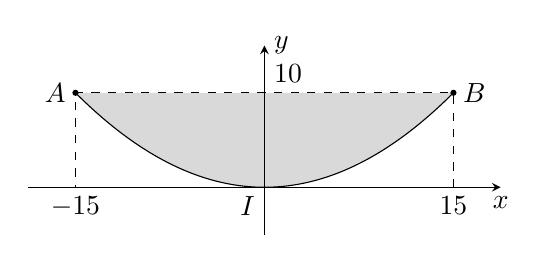
\begin{tikzpicture}[smooth,samples=300,scale=0.6,>=stealth]
				\fill[gray!30] (-4,2)--(4,2)--plot[domain=4:-4](\x,{0.125*(\x)^2});
				\draw[->] (-5,0)--(5,0) node[below]{$x$};
				\draw[->] (0,-1)--(0,3) node[right]{$y$};
				\draw (0,0) node[below left]{$I$};
				\draw[domain=-4:4] plot(\x,{0.125*(\x)^2});
				\draw[fill=black] (4,2) circle(1.5pt) (-4,2) circle(1.5pt);
				\draw[dashed] (4,0)node[below]{$15$}--(4,2)node[right]{$B$}--(-4,2)node[left]{$A$}--(-4,0)node[below]{$-15$};

				\node[right] at (0,2.4) {$10$};
			\end{tikzpicture}}
		\noindent
		Vậy $y=\dfrac{2}{45}x^2$. Diện tích phần tô đen là $S=2 \cdot \displaystyle\int\limits_{-15}^{15} \left(10-\dfrac{2}{45}x^2 \right) \mathrm{\,d}x=400 \, (\text{m}^2)$.\\
		Diện tích phần còn lại của sân bóng là $S_2=30 \cdot 50-400=1100\,(\text{m}^2).$\\
		Số tiền Ông An phải trả để trồng cỏ nhân tạo cho sân bóng là
		\[130000\times 400+90000\times 1100=151000000\text{ đồng}=151\text{ triệu đồng.}\]}
\end{ex}

% \Closesolutionfile{ansbook}
% \HetDe
% \label{De1}
% %
% \cleardoublepage
% \setcounter{page}{1}
% \rfoot{Trang \thepage/\pageref{DA1} - Đáp án trắc nghiệm Mã đề 1}
% \begin{center}
% 	\bfseries ĐÁP ÁN TRẮC NGHIỆM MÃ ĐỀ 1
% \end{center}

% \inputansbox{10}{ans/ansDe1-TN1}
% \inputansbox[3]{2}{ans/ansDe1-TN2}
% \inputansbox{3}{ans/ansDe1-TN3}
% \label{DA1}
% %
